%%%%(c) COPYRIGHT NOTICE%FOLDUP
%%%%(c)
%%%%(c)  This file is a portion of the source for the textbook
%%%%(c)
%%%%(c)    Numerical Methods Course Notes,
%%%%(c)    Copyright 2004-2010 by Steven E. Pav
%%%%(c)
%%%%(c)  See the file COPYING.txt for copying conditions
%%%%(c)
%%%%(c)%UNFOLD
\documentclass[11pt]{book}
\textheight=9in\textwidth=6.5in\topmargin=-.25in\oddsidemargin=0in\evensidemargin=0in

\makeindex 

%%throat clearing%FOLDUP
\typeout{-- numas.tex}
\typeout{-- quadrature.tex}
\typeout{-- N� 2004-2010 Steven E. Pav}
%UNFOLD

%%local commands%FOLDUP
%UNFOLD

\usepackage{empheq}
\usepackage{makeidx}
\usepackage{graphicx,epsfig,psfrag}
\usepackage{subfigure}
\graphicspath{{figs/}}
\usepackage{alg}

\usepackage[newitem,newenum,increaseonly]{paralist}
\usepackage{import}

\usepackage[environments,commands,meshstuff,shortcuts]{sepmath}

%\numberwithin
\newtheorem{bktheorem}{Theorem}[chapter]
\newtheorem{bkcorollary}[bktheorem]{Corollary}
\newtheorem{bkexample}[bktheorem]{Example}
\newtheorem{bkexprob}[bktheorem]{Example Problem}
\newtheorem{bkdefinition}[bktheorem]{Definition}
\newtheorem{bkexercise}{Exercise}[chapter]
\newtheorem{bkproblem}[bkexercise]{Problem}

\providecommand{\bkthmref}[1]{Theorem~\ref{bkthm:#1}}
\providecommand{\bkexref}[1]{Example~\ref{bkex:#1}}
\providecommand{\bkexpref}[1]{Example Problem~\ref{bkexp:#1}}
\providecommand{\chexref}[2][\thechapter]{Exercise~({#1}.\ref{chex:#2})}
\providecommand{\octmat}{octave/Matlab\xspace}

%\vspace*{10mm}
%\pagebreak[4]
\newenvironment{bkexs}{%
\clearpage
\begin{center}\framebox[0.95\columnwidth][s]{\sc Exercises\hfill}\end{center}
\vspace{-1mm}
\addcontentsline{toc}{section}{Exercises}
\begin{compactenum}[({\thechapter}.1)]
%[{\bf\thechapter.\enumi}]
}{%
\end{compactenum}
}
\newenvironment{bksolution}{%
\\\emph{Solution:} %
}{%
\hfill$\dashv$%
}
\newenvironment{bkhint}{%
(\emph{Hint:} %
}{%
)}
\newenvironment{bknote}{%
(\emph{Note:} %
}{%
)}

\providecommand{\widefbox}[1]{\fbox{\hspace{1em}{#1}\hspace{1em}}}
%to note the dependencies between chapters; a hack
\providecommand{\depson}[2]{\typeout{DEP: "\ref{#1}" -> "\ref{#2}"}}

%%%%%%%%%%%%%%%%%%%%%%%%%%%%%%%%%%%%%%%%%%%%%%%%%%%%%%%%%%%%%%%%%%%%%%

\title{Numerical Methods Course Notes\\Version 0.11\\(UCSD Math 174, Fall 2004)}%FOLDUP
\author{Steven E. Pav\thanks{Department of Mathematics, MC0112, University of
California at San Diego, La Jolla, CA 92093-0112.
%$\left<\mathtt{spav@ucsd.edu}\right>$
\texttt{<spav@ucsd.edu>}
This document is Copyright \copyright{} 2004-2006 Steven E. Pav.  
Permission is granted to copy, distribute and/or modify this document
under the terms of the GNU Free Documentation License, Version 1.2
or any later version published by the Free Software Foundation;
with no Invariant Sections, no Front-Cover Texts, and no Back-Cover
Texts.  A copy of the license is included in the section entitled "GNU
Free Documentation License".}}
\date{\today}
%UNFOLD

\begin{document}
%%%%%%%%%%%%%%%%%%%%%%%%%%
\maketitle
\frontmatter

\chapter*{Preface} %FOLDUP
\addcontentsline{toc}{chapter}{Preface}
These notes were originally prepared during Fall quarter 2003 for UCSD Math
174, Numerical Methods.  In writing these notes, it was not my intention to add
to the glut of Numerical Analysis texts; they were designed to complement the 
course text, 
\emph{Numerical Mathematics and Computing,} Fourth edition, by Cheney and
Kincaid \cite{KdCw1999}.  As such, these notes follow the conventions of that
text fairly closely.  If you are at all serious about pursuing study of
Numerical Analysis, you should consider acquiring that text, or any one of a
number of other fine texts by \eg Epperson, Hamming, etc. 
\cite{Ejf2001,Hr1987,IeKhb1966}.

%\figref{depgraph}%FOLDUP
\begin{figure}[htb!]
\centering
	\includegraphics[width=0.75\columnwidth,angle=0,clip=]{numas.dep.eps}
\caption{The chapter dependency of this text, though some dependencies are weak.}\label{fig:depgraph}
\end{figure}%UNFOLD

Special thanks go to the students of Math 174, 2003--2004, who suffered through
early versions of these notes, which were riddled with (more) errors.

\section*{Revision History}
\begin{compactenum}
\item[0.0] Transcription of course notes for Math 174, Fall 2003.
\item[0.1] As used in Math 174, Fall 2004.
\item[0.11] Added material on functional analysis and Orthogonal Least Squares.
\end{compactenum}

\section*{Todo}
\begin{compactitem}
\item More homework questions and example problems.
\item Chapter on optimization.
\item Chapters on basic finite difference and finite element methods?
\item Section on root finding for functions of more than one variable.
\end{compactitem}

%UNFOLD

\tableofcontents

%%%%%%%%%%%%%%%%%%%%%%%%%%
\mainmatter

%%the chapters%FOLDUP
\import*{./}{intro}
\import*{./}{matlab}
\import*{./}{linearsys}
\import*{./}{rootfind}
\import*{./}{interpolate}
\import*{./}{splines}
\import*{./}{derivatives}
\import*{./}{quadrature}
\import*{./}{leastsquares}
\import*{./}{odes}
%these are only stubs right now;
%\import*{./}{fdm}
%\import*{./}{fem}
%UNFOLD

\appendix
\import*{./}{oldexams}
%\small
\footnotesize
\scriptsize
\import*{./}{fdl}
\normalsize

\nocite{MR97g:65003,Bag2002}
%%%%%%%%%%%%%%%%%%%%%%%%%%
\backmatter

%FOLDUP
\bibliographystyle{sepbib}
\addcontentsline{toc}{chapter}{Bibliography}
\bibliography{numas}
\printindex

%\section{Code}\label{sec:code}
%\input{allcode}
%UNFOLD
\end{document}
%for vim modeline: (do not edit)
% vim:ts=2:sw=2:tw=79:fdm=marker:fmr=FOLDUP,UNFOLD:cms=%%s:tags=tags;:syntax=tex:filetype=tex:ai:si:cin:nu:fo=croqt:cino=p0t0c5(0:
